\subsection{Early signals of sterile neutrinos}
Despite the success of three-flavor oscillation model in explaining the data from solar, atmospheric, reactor and accelerator experiments, there is a mess related to the results from the SBL accelerator experiments. The signals from these experiments indicated oscillations induced by a mass squared gap around the order of 1~eV$^2$. This gap is not compatible with the well-established solar and atmospheric mass squared gaps. This fact, in turn, implies the presence of at least one new neutrino state, which was contemplated to possibly mix with the other three states. However, the constraint on the number of active neutrinos, precisely set by LEP experiments, renders the new state(s) a sterile neutrino(s), which means forbidding this state(s) to involve in the weak interaction.\\

A number of models are threw into the field in order to absorb the new data into the already constructed neutrino oscillation framework. A few candidates to name are 3+1, 3+2 and 3+3. Models such as 2+2 or 3+1+1 were highly disfavored by either cosmological or short baseline oscillation data. In this note, we will primarily discuss the 3+1 model, in which, one light sterile neutrino (1~eV) is added to the particle content.

\subsubsection{The LSND experiment}
LSND, short for \textbf{L}iquid \textbf{S}cintillator \textbf{N}eutrino \textbf{D}etector, is a tank filled with 167 tons of mineral oil that was doped with 6.4~kg of b-PDB organic scintillator. Scintillation and Cherenkov lights were collected using an array of 1220 photomultipliers surrounding the tank. The detector was placed 30~m away from the beam stop \cite{ATHANASSOPOULOS1997149}.\\

The beamline utilized in the experiment is a 798~MeV proton beam directed onto a target at a duty factor of $6\times 10^{-2}$, producing pions and muons that decay at rest into a beam of muon antineutrinos with the energy of 20-200~MeV, peaking at around 50~MeV \cite{PhysRevD.64.112007}, just like the interactions mentioned in \eqref{eq:piKdecay} and \eqref{eq:mudecay}. The $ \pi^- $ decay is strongly suppressed due to the pion capture on target nuclei. This led to a low ratio of flux between the intrinsic $ \bar{\nu}_e $ and the $ \bar{\nu}_\mu $.\\

The $ \bar{\nu}_e $ in the beam, no matter being an intrinsic component or oscillated product, can be detected via inverse beta decay
\begin{equation}
	\bar{\nu_e} + p \rightarrow e^+ + n,
\end{equation}
which results in clear signals from positron annihilation companied by a 2.2~MeV gamma from neutron capture. \\
%Consider adding this if necessary: One feature of LSND detector is to measure energy and angle of the produced positron thanks to the ability to reconstruct the Cherenkov light emitted.\\

With the energy lower than the CC interaction threshold, the $ \bar{\nu}_\mu $ and $ \nu_\mu $ in LSND are detected mainly in NC channel. Lastly, the $ \nu_e $ in the beam is detected in
\begin{equation}
	\nu_e + ^{12}\text{C} \rightarrow~ ^{12}\text{N} + e^-.
\end{equation}
This is hardly misidentified as inverse beta decay signal because there is no associated neutron capture.\\

%On the physics results, a clear excess of electron antineutrinos was observed as an evidence for neutrino oscillations. However, the corresponding mass-squared gap is nearly 1~eV$^2$, casting doubts on the three-flavor model, which was supported by later experiments, namely Super-K, KamLAND or SNO. Simply put, LNSD signals cannot be explained in the framework of only three neutrino flavors: at least one more neutrino with the mass close to 1~eV need to be added.
The LSND result can be interpreted as a 3$ \sigma $ signal of $ \bar{\nu}_\mu \rightarrow \bar{\nu}_e $. The corresponding mass-squared gap is nearly 1~eV$^2$, thus might cast doubts on the three-flavor model which was supported by later experiments, namely Super-K, KamLAND or SNO. However, the signals seen in LNSD have not been confirmed in Karmen, which is also an SBL with similar sensitivity and somewhat shorter baseline, $ L=18~$m. 

\subsubsection{The MiniBooNE experiment}
Constructed as a test of LNSD results, MiniBooNE came into operation with the presumptions that the physics behind LNSD signals depends only on $ L/E $ ratio and respects the $ CP $ symmetry.\\

MiniBooNE, in contrast to LNSD, exploited a conventional neutrino beamline. High energy protons are directed to a beryllium target then produces mesons, mainly pions and kaons, that successively selected by magnetic fields and decay-in-flight to neutrinos or antineutrinos. In the $ \nu_\mu $ mode, the beam energy was around 5~GeV, peaking at about 0.6~GeV, with a negligible amount of $\bar{\nu}_\mu $, $ \bar{\nu}_e $ and $ \nu_e $ contaminated. In the $ \bar{\nu}_\mu $ mode, the contamination of $ \nu_\mu $ becomes significant and above 2~GeV, even dominates the beam \cite{AguilarArevalo200928}. In all, the beam is quite versatile and it handed MiniBooNE an advantage over LSND of probing the disappearance probability for both neutrinos or antineutrinos, thus measuring possible $ CP $ violation effects.\\

The detector was a spherical tank filled with 806 tons of $\text{C}\text{H}_2 $ without scintillator doping, and located 541~m downstream of the target \cite{AguilarArevalo200928}. The signals were recored using 1280 8-inch PMTs.\\

In the energy range provided for MiniBooNE, most of the contribution to CC cross sections comes from the quasi-elastic scattering and single pion production. The detection targets are mainly the nucleons in carbon and hydrogen atoms. The signals are recognized by the patterns of observed Cherenkov rings, see Fig. \ref{fig:mbtopology}. \\

\begin{figure}[h!]
	\begin{center}
		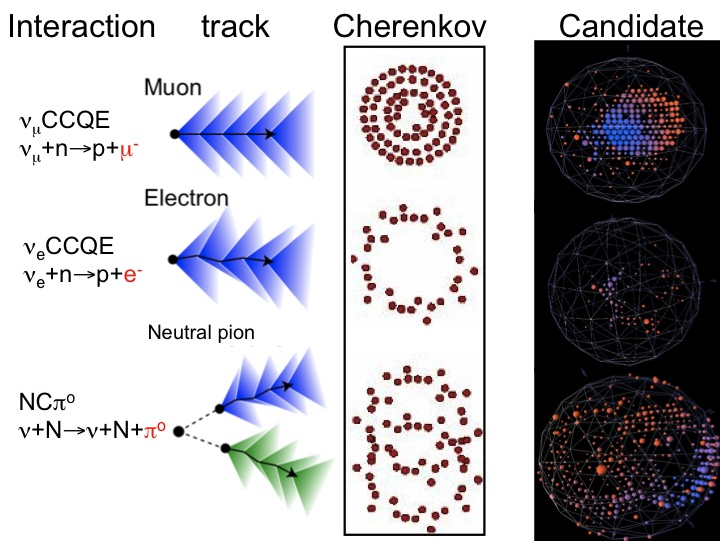
\includegraphics[scale=0.3]{MB_topology}
		\caption{The particle identification based on Cherenkov ring's topologies. From left to right, interaction types, characteristics of tracks and Cherenkov rings, and event displays of candidate events.}
	\end{center}
	\label{fig:mbtopology}
\end{figure}

An excellent review on LSND and MiniBooNE and their physics implication can be found in \cite{annurev-nucl-102711-094957}.





